\documentclass[12pt]{article}
\setlength{\oddsidemargin}{0in}
\setlength{\evensidemargin}{0in}
\setlength{\textwidth}{6.5in}
\setlength{\parindent}{0in}
\setlength{\parskip}{\baselineskip}

\usepackage{amsmath,amsfonts,amssymb,bm,graphics,pgfplots,framed,dsfont}
\usepgfplotslibrary{fillbetween} % Load the fillbetween library
\usepackage[scale=0.75,top=1cm,bottom=3cm]{geometry}

\begin{document}

\textbf{Minh Anh Nguyen }\\
\textbf{Calculus 1 Assignment-12}\\
\textbf{Section: 04}\\
\textbf{TA's name: Arthur Huey}

\hrulefill

Section 5.1:

\begin{enumerate}
\setcounter{enumi}{1}
    \item Let:
    \begin{center}
        \includegraphics{img/img-0.png}
    \end{center}
    \begin{enumerate}
        \item Set up an integral for the area of the shaded region.
        \[\int_{1}^{4} (\sqrt{x} - \frac{1}{x^2})dx\]
        \item Evaluate the integral to find the area.
        \[\int_{1}^{4} (\sqrt{x} - \frac{1}{x^2})dx = \int_{1}^{4} (x^{1/2} - x^{-2})dx = (\frac{2x^{3/2}}{3} + \frac{1}{x})|_{1}^{4} = \frac{67}{12} - \frac{5}{3} = \frac{47}{12}\]
    \end{enumerate}

\setcounter{enumi}{3}
    \item Let:
    \begin{center}
        \includegraphics{img/img-1.png}
    \end{center}
    \begin{enumerate}
        \item Set up an integral for the area of the shaded region.
        \[\int_{0}^{3}(y^2-4y-2y+y^2)dy = \int_{0}^{3}(2y^2-6y)dy \]
        \item Evaluate the integral to find the area.
        \[\int_{0}^{3}(2y^2-6y)dy = (\frac{2y^3}{3}-3y)|_{0}^{3} = 9 - 0 = 9\]
    \end{enumerate}

\setcounter{enumi}{6}
    \item Set up, but do not evaluate, an integral representing the area of the region enclosed by the given curves.
    \[y = \frac{1}{x},y = \frac{1}{x^2},x=2\]
    \[\int_{0}^{2}|\frac{1}{x} - \frac{1}{x^2}|dx\]

\setcounter{enumi}{11}
    \item Sketch the region enclosed by the given curves. Decide whether to integrate with respect to $x$ or $y$. Draw a typical approximating rectangle and label its height and width. Then find the area of the region.
    \[y = 1 + x^3,y = 2-x,x=-1,x=0\]
    \begin{center}
        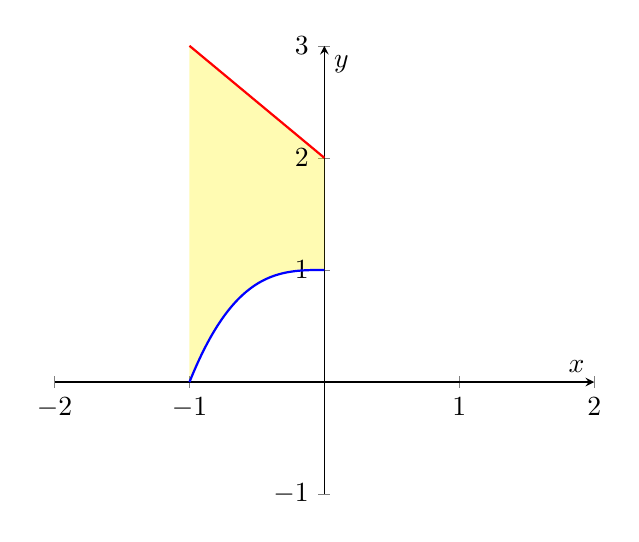
\begin{tikzpicture}
            \begin{axis}[
                axis lines = middle,
                xlabel = $x$,
                ylabel = $y$,
                xmin = -2, xmax = 2,
                ymin = -1, ymax = 3,
                samples = 100,
                domain = -1:0,
                legend pos = north east,
                legend style = {draw=none}
            ]

            % Shading the enclosed area
            \addplot [
                name path=A,
                domain=-1:0,
                thick,
                draw=none
            ] {1 + x^3};

            \addplot [
                name path=B,
                domain=-1:0,
                thick,
                draw=none
            ] {2 - x};

            % Fill the area between the two functions
            \addplot [
                fill=yellow, fill opacity=0.3
            ] fill between[of=A and B];

            % Plot y = 1 + x^3
            \addplot[blue, thick] {1 + x^3};

            % Plot y = 2 - x
            \addplot[red, thick] {2 - x};

            \end{axis}
        \end{tikzpicture}
    \end{center}
    \[\int_{-1}^{0}(2-x-1-x^3)dx = \int_{-1}^{0}(-x^3-x+1) = (-\frac{x^4}{4}-\frac{x^2}{2} + x)|_{-1}^{0} = \frac{7}{4}\]

\setcounter{enumi}{21}
    \item Sketch the region enclosed by the given curves and find its area.
    \[y = \sqrt{x-1},x-y = 1\]    
    \begin{center}
        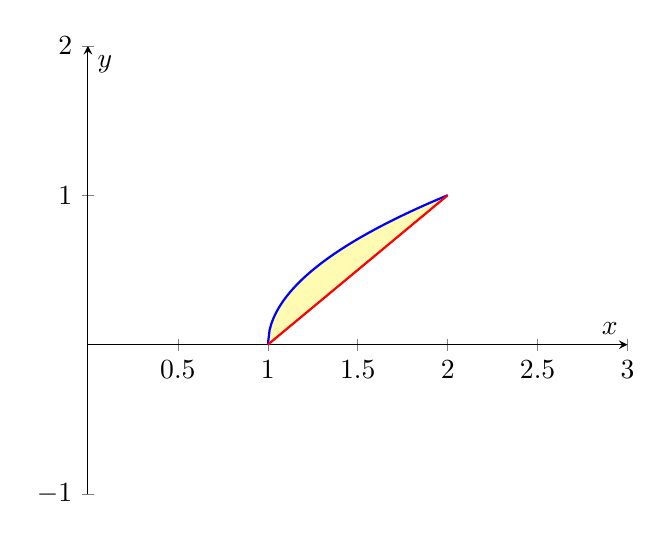
\begin{tikzpicture}
            \begin{axis}[
                axis lines = middle,
                xlabel = $x$,
                ylabel = $y$,
                xmin = 0, xmax = 3,
                ymin = -1, ymax = 2,
                samples = 100,
                domain = 1:2,
                legend pos = north east,
                legend style = {draw=none}
            ]

            % Define the path for y = sqrt(x - 1) from x = 1 to x = 2
            \addplot [
                name path=A,
                domain=1:2,
                thick,
                draw=none
            ] {sqrt(x - 1)};

            % Define the path for x - y = 1, rearranged as y = x - 1, from x = 1 to x = 2
            \addplot [
                name path=B,
                domain=1:2,
                thick,
                draw=none
            ] {x - 1};

            % Fill the area between the two paths
            \addplot [
                fill=yellow, fill opacity=0.3
            ] fill between[of=A and B];

            % Plot y = sqrt(x - 1)
            \addplot[blue, thick] {sqrt(x - 1)};

            % Plot x - y = 1 (or y = x - 1)
            \addplot[red, thick] {x - 1};

            \end{axis}
        \end{tikzpicture}
    \end{center}
    \[x-y=1 \rightarrow y = x - 1\]
    \[\int_{1}^{2}(\sqrt{x-1}-x+1)dx = \frac{1}{6}\]

\setcounter{enumi}{35}
    \item Sketch the region enclosed by the given curves and find its area.
    \[y = \frac{x}{\sqrt{1+x^2}}, y = \frac{x}{\sqrt{9-x^2}}, x\geq 0\]
    \begin{center}
        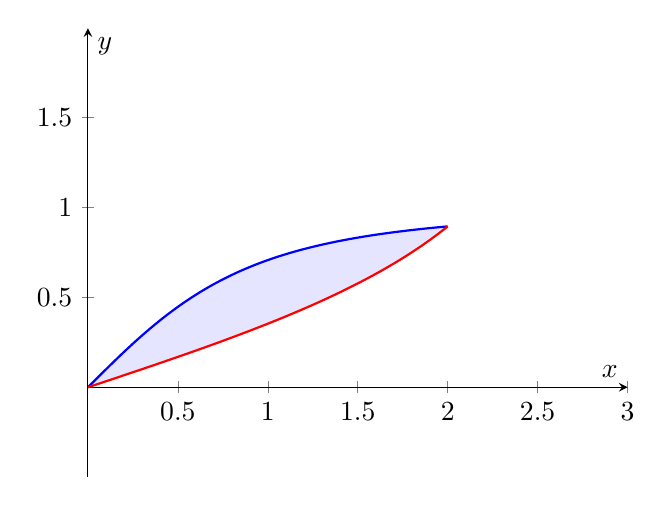
\begin{tikzpicture}
            \begin{axis}[
                axis equal,
                axis lines=middle,
                xlabel={$x$},
                ylabel={$y$},
                xmin=0, xmax=3,
                ymin=0, ymax=1.5,
                samples=100,
                domain=0:2,
                legend pos=north east
            ]
            
            % Plot the first curve y = x / sqrt(1 + x^2)
            \addplot[name path=A, blue, thick] {x / sqrt(1 + x^2)};
            
            % Plot the second curve y = x / sqrt(9 - x^2)
            \addplot[name path=B, red, thick] {x / sqrt(9 - x^2)};
        
            % Fill the enclosed region between the two curves
            \addplot[blue!20, opacity=0.5] fill between[of=A and B, soft clip={domain=0:3}];
            
            \end{axis}
        \end{tikzpicture}
        \[\int_{0}^{2}(\frac{x}{\sqrt{1+x^2}}-\frac{x}{\sqrt{9-x^2}})dx = \int_{0}^{2}(\frac{x}{\sqrt{1+x^2}})dx-\int_{0}^{2}(\frac{x}{\sqrt{9-x^2}})dx\]
        First Integral: \(\int_{0}^{2} \frac{x}{\sqrt{1 + x^2}} dx\)
        Let \( u = 1 + x^2 \), then \( du = 2x \, dx \) or \( dx = \frac{du}{2x} \).
        \[\int \frac{x}{\sqrt{1 + x^2}} dx = \int \frac{x}{\sqrt{u}} \cdot \frac{du}{2x} = \int \frac{1}{2 \sqrt{u}} \, du = \frac{1}{2} \int u^{-\frac{1}{2}} \, du\]
        \[= \frac{1}{2} \cdot 2\sqrt{u} = \sqrt{u} = \sqrt{1 + x^2}\]
        \[\int_{0}^{2} \frac{x}{\sqrt{1 + x^2}} dx = \left[ \sqrt{1 + x^2} \right]_{0}^{2} = \sqrt{5} - 1\]
        Second Integral: \(\int_{0}^{2} \frac{x}{\sqrt{9 - x^2}} dx\)
        Let \( u = 9 - x^2 \), then \( du = -2x \, dx \) or \( dx = \frac{-du}{2x} \).
        \[\int \frac{x}{\sqrt{9 - x^2}} dx = \int \frac{x}{\sqrt{u}} \cdot \frac{-du}{2x} = -\frac{1}{2} \int u^{-\frac{1}{2}} \, du\]
        \[= -\frac{1}{2} \cdot 2\sqrt{u} = -\sqrt{u} = -\sqrt{9 - x^2}\]
        \[\int_{0}^{2} \frac{x}{\sqrt{9 - x^2}} dx = \left[ -\sqrt{9 - x^2} \right]_{0}^{2} = -( \sqrt{5} - 3) = 3 - \sqrt{5}\]
        Final Answer
        \[\int_{0}^{2} \left( \frac{x}{\sqrt{1 + x^2}} - \frac{x}{\sqrt{9 - x^2}} \right) dx = (\sqrt{5} - 1) - (3 - \sqrt{5}) = 2\sqrt{5} - 4\]
    \end{center}

\setcounter{enumi}{63}
    \item Question:
    \begin{enumerate}
        \item Find the number $a$ such that the line $x=a$ bisects the area under the curve $y=\frac{1}{x^2}$, $1 \leq x \leq 4$.\\
        The area of the region under the curve  $y=\frac{1}{x^2}$, $1 \leq x \leq 4$ is:
        \[\int_{1}^{4} \frac{1}{x^2} = (-\frac{1}{x})|_1^4 = (-\frac{1}{4} + \frac{1}{1}) = \frac{3}{4}\]\
        \[\int_{1}^{a} \frac{1}{x^2} = (-\frac{1}{x})|_1^a = (-\frac{1}{a} + \frac{1}{1}) = \frac{3}{8}\]
        \[-\frac{1}{a} = -\frac{5}{8}\]
        \[a = \frac{8}{5}\]
        \item Find the number $b$ such that the line $y=b$ bisects the area in part (a).\\
        The area of the region under the curve  $x=\frac{1}{\sqrt{y}}$, $1 \geq y \geq \frac{1}{16}$ is:
        \[\int_{1/16}^{1} \frac{1}{\sqrt{y}}dy = (2\sqrt{y})|_{1/16}^{1} = (2 - \frac{1}{4}) = \frac{3}{4}\]
        \[\int_{1/16}^{b} \frac{1}{\sqrt{y}}dy = (2\sqrt{y})|_{1/16}^{b} = (2 - \frac{1}{\sqrt{b}}) = \frac{3}{8}\]    
        \[ - \frac{1}{\sqrt{b}} = -\frac{13}{8}\]
        \[b = \frac{64}{169}\]
    \end{enumerate}
    
\end{enumerate}

Section 5.2:

\begin{enumerate}
\setcounter{enumi}{1}
    \item A solid is obtained by revolving the shaded region about the specified line.
    \begin{center}
        \includegraphics{img/img-2.png}
    \end{center}
    About the $x$-axis.
    \begin{enumerate}
        \item Sketch the solid and a typical disk or washer.
        \item Set up an integral for the volume of the solid.
        \[\int_{0}^{4}(\sqrt{x} - \frac{1}{2}x)dx \]
        \item Evaluate the integral to find the volume of the solid.
        \[\int_{0}^{4}(\sqrt{x} - \frac{1}{2}x)dx = (\frac{2x^{3/2}}{3} - \frac{1}{4}x^2)|_0^4 = \frac{4}{3}\]
    \end{enumerate}
    \item A solid is obtained by revolving the shaded region about the specified line.
    \begin{center}
        \includegraphics{img/img-3.png}
    \end{center}
    About the $y$-axis.
    \begin{enumerate}
        \item Sketch the solid and a typical disk or washer.
        \item Set up an integral for the volume of the solid.
        \[\int_{1}^{9} (9 - \sqrt[3]{y-1})dy \]
        \item Evaluate the integral to find the volume of the solid.
        \[\int_{0}^{4}(\sqrt{x} - \frac{1}{2}x)dx = (\frac{2x^{3/2}}{3} - \frac{1}{4}x^2)|_0^4 = \frac{4}{3}\]
    \end{enumerate}
\end{enumerate}
\end{document}


